\chapter{Conceitos}
\label{cap:conceitos}

Este capítulo está dividido em várias seções, a saber: a primeira seção identifica o panorama dos paradigmas de produção considerando os períodos conhecidos como 1ª, 2ª e 3ª revoluções industriais, bem como identifica alguns pontos que evidenciam a 4ª Revolução Industrial; a segunda seção apresenta um estudo específico sobre EPS, que é o paradigma deste trabalho; a terceira seção mostra a conceituação teórica de alguns termos importantes para o entendimento do assunto; e a última seção identifica as pesquisas e trabalhos que se configuram como o estado da arte em sistemas baseados no paradigma evolutivo.



%===================================================================

\section{Panorama dos paradigmas de produção até os dias atuais}	

\subsection{Revoluções industriais}

A Figura \ref{F9} ilustra um breve panorama do período iniciado com a primeira revolução industrial até o futuro próximo. Nela, nota-se que, após o período feudal, o nascimento da Primeira Revolução Indústria, onde a produção artesanal (realizada por máquinas artesanais) perde espaço para a produção em massa (produção de lotes grandes e realizada por máquinas mecânicas) da indústria mecânica da Segunda Revolução Industrial. Com o advento da Terceira Revolução Industrial passe a produzir lotes médios através das máquinas flexíveis. 

O problema da personalização de produtos surge também nessa época. Para tratar tal problema, surgem máquinas ágeis (baseada nos paradigmas BMS, RMS e HMS, detre outros) e esta fase é aqui identificada com indústria híbrida. Nos dias atuais surge o fenômeno da customização em massa e, para lidar com os lotes pequenos e a alta variabilidade destes, surgem os sistemas emergentes baseados nos paradigmas EAS/EPS e a auto-organização. A chamada Quarta Revolução Industrial, a caminho, é baseada principalmente nos paradigmas ágeis e evolutivos de produção. 

Nesta seção são evidenciados o surgimento dos paradigmas e comentados alguns conceitos surgidos após esse período.

%==================================================================
\begin{figure}
	\centering
	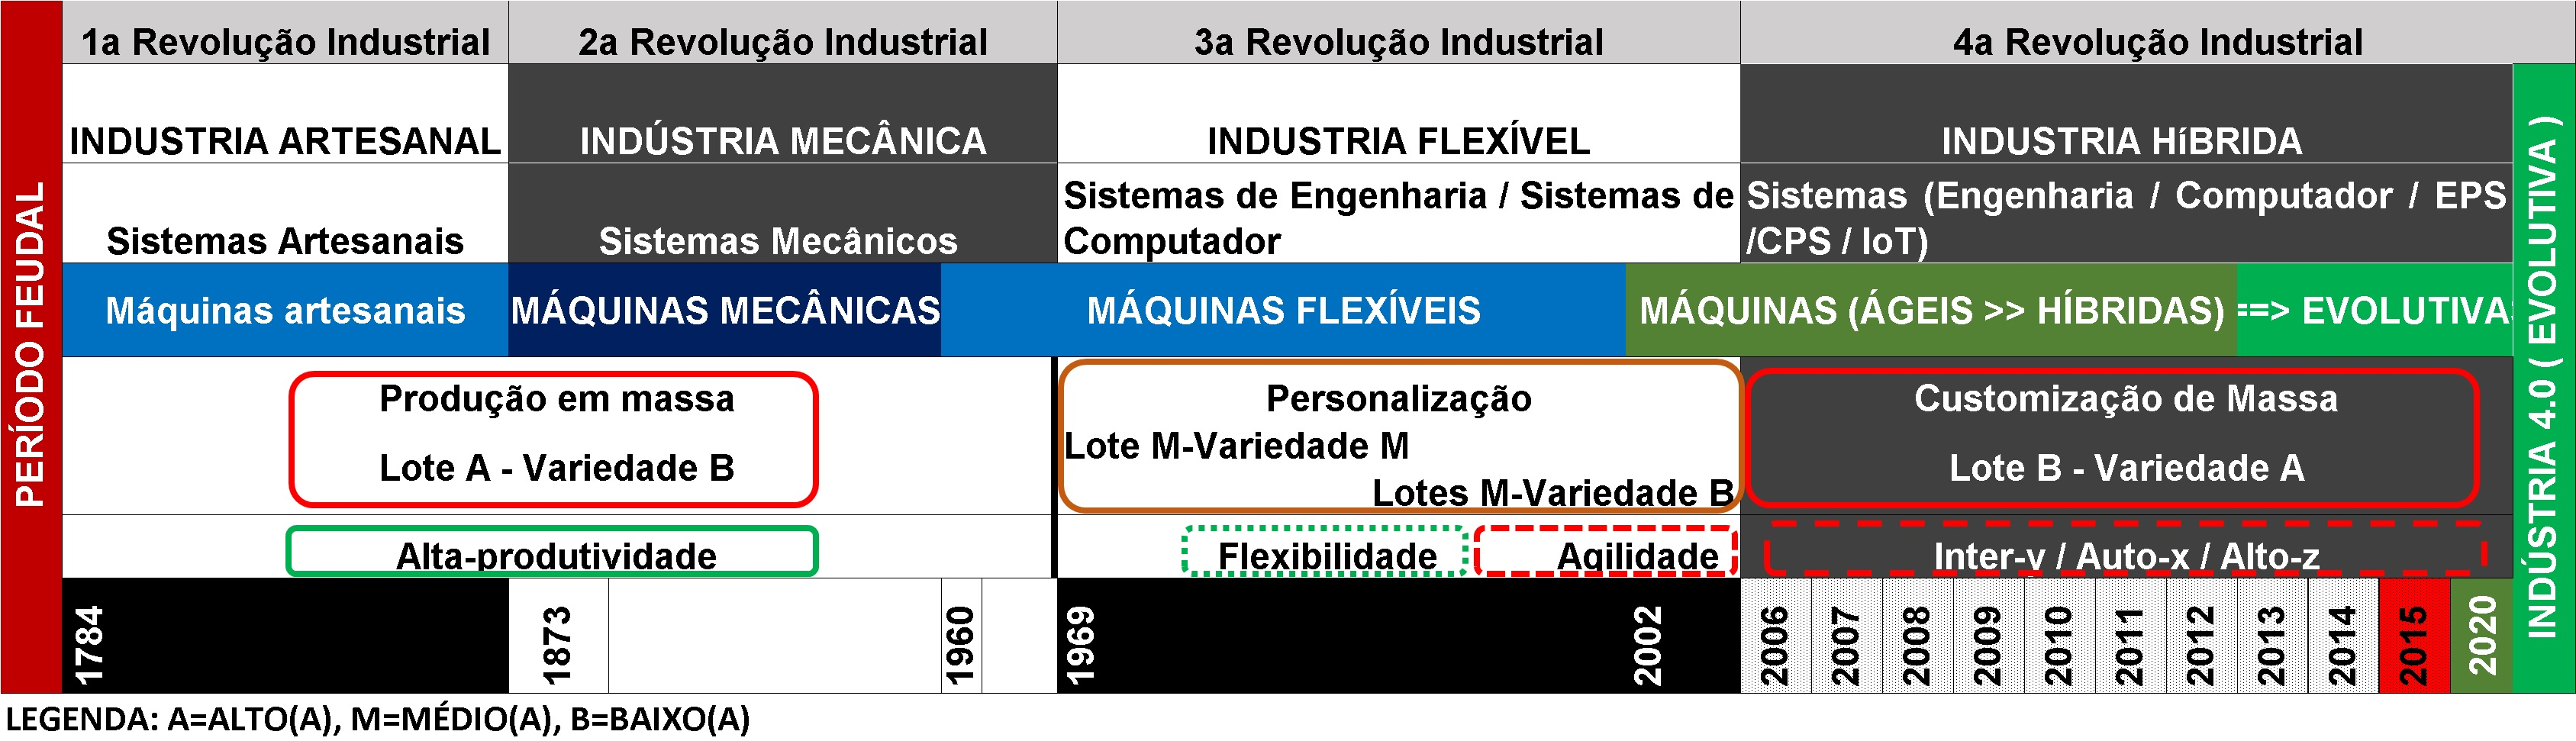
\includegraphics[width=16cm, height=6cm]{img/F9_MeDSE_RI_FULL3.jpg} 
	\caption{Revoluções Industriais, problemas e soluções}
	%{\footnotesize{Fonte: \cite{KOREN1999}}}
	\label{F9}
\end{figure}
%==================================================================

\subsection{Da máquina de Heron às máquinas flexíveis}	

Desde que os processos manuais artesanais foram substituídos por processos industriais, com o advento da Revolução Industrial, avanços tecnológicos têm causado mudanças no sistema de produção \cite{NAHER2008}. Com o advento da \textit{máquina a vapor}, um melhoramento da \textit{Máquina de Heron}, e a criação do tear mecânico, por volta de 1784, teve início o período conhecido como a $1^a$ Revolução Industrial, período no qual relevantes avanços científicos e sociais foram conseguidos naquela sociedade advinda de um sistema de feudos. Durante esse período a indústria ficou conhecida por suas características ainda artesanais como Indústria Artesanal. Esse período durou até o surgimento da eletricidade em 1873, fato que marcou o início da $2^a$ Revolução Industrial e a indústria passou de artesanal para mecânica. Nessa Indústria Mecânica, elevados lotes de produção foram conseguidos para atender às massas, que foram uma crescente demanda na Europa e nas Américas \cite{DRATH2014}

A Indústria Mecânica deu lugar à Indústria Flexível devido aos avanços tecnológicos conseguidos a partir de 1969 no campo da Eletrônica, em especial a  produção do primeiro controlador lógico programável (PLC) e significativos avanços na Tecnologia da Informação \cite{NAHER2008}.



\subsection{O surgimento dos sistemas flexíveis baseados no paradigma \textit{FMS}}	

Com a continuidade do desenvolvimento tecnológico, as máquinas flexíveis foram integradas e transformaram-se em sistemas e mostraram uma nova maneira de aumentar a produtividade, isso no ano de 1967 \cite{KOREN1999}.

Na Alemanha, em 1969, os sistemas \textit{Flexible Manufacturing System (FMS)}  foram instalados na empresa \textit{Heildlenberger Druckmaschinen} com a cooperação da Universidade de \textit{Stuttgart}. Em 1972 na exposição de \textit{Stanki} os sistemas \textit{FMS} foram demonstrados para os russos. O Japão teve seu primeiro \textit{FMS} em 1985 instalado na \textit{Fuji Xerox} \cite{GROOVER2011}. 

O trabalho desenvolvido por \citeonline{ELMARAGHY1982} deixou claro como os sistemas \textit{FMS} foram utilizados para resolver o problema da produtividade dos lotes de volume médio mas que começavam a se apresentar recheados de variedades, o que aumentava os custos e reduzia os lucros. Como o sistema produtivo \textit{FMS} podia ser, além de reprogramado, reconfigurado, este permitiu a produção de produtos sob demanda em médias quantidades, com melhores custos, e a indústria passou, então, a colocar no mercado produtos personalizados, ou seja, seguindo as preferências do cliente. Com a constante utilização de sistemas \textit{FMS}, logo se percebeu que a solução proposta para os lotes médios já não tinha a mesma eficácia. Quando essas quantidades tendiam a valores menores, a personalização de produtos passou a ser um problema. 

Neste texto, o termo \textit{personalização} é utilizado para representar um nível menor de \textit{customização}. A \textit{customização} é caracterizada por uma produção variada de produtos com curtos ciclos de vida~\cite{QUINTELA2005}.

\subsection{O surgimento dos sistemas emergentes baseados em \textit{BMS}, \textit{HMS} e \textit{RMS}}

Para enfrentar os desafios da agilidade e urgência impostos pela personalização, foi proposto por Ueda o paradigma \textit{Bionic Manufacturing System (BMS)}~\cite{UEDA1992}, que inspirou-se nos sistemas biológicos para realizar analogias com o  sistema produtivo e propor uma solução para a personalização. 

Ainda na década de 90, surge o paradigma \textit{Holonic Manufacturing System (HMS)}~\cite{CHRISTENSEN1994,VANBRUSSEL1998}  que considerou para suas análises, o sistema produtivo como um sistema composto por \textit{holons} que trocavam informações entre si. 

Ao final da década de 90, pode-se perceber um novo paradigma: \textit{Reconfigurable Manufacturing System (RMS)}~\cite{KOREN1999}, que prometia sistemas capazes de serem reconfiguráveis no chão-de-fábrica, cujos componentes eram máquinas e controladores reconfiguráveis, elaborados com metodologias para uma concepção sistemática e reposta rápida às exigências das bruscas alterações de demanda nos mercados globalizados.
 
Com o aumento da personalização possibilitado pelos sistemas \textit{FMS}, os consumidores passaram a exigir essa personalização para outros tipos de produtos, refletindo um aumento das exigências dos clientes. A tendência se concretizou e a fabricação de produtos sob medida, refletindo a preferência do cliente, passou a ser lugar comum nos mercados globalizados, e o fenômeno recebeu o nome de customização em massa \cite{DAVIS1997}, pois além de produzir o produto, o produtor deveria atender às especificações de qualidade definidas pelo usuário do produto. 

Mais recentemente, nos anos 2000 foi proposto, por Onori o paradigma \textit{Evolvable Assembly System (EAS)}~\cite{ONORI2002,FREI2006} que serviu de base para o paradigmas \textit{Evolvable Production System (EPS)}~\cite{ONORI2010}. O paradigma \textit{EPS} utiliza o conceito de agentes inteligentes para realizar as operações dentro do sistema produtivo. EPS permite a implementação de um sistema que atende a duas das características desejadas na manufatura: auto-organização e auto-otimização. Estas por sua vez permitem a produção de produtos diferentes, não necessariamente definidos com o processo produtivo, e a otimização do uso de alguns dos recursos do sistema.

%Essas soluções buscam sistemas com características de flexibilidade, agilidade, interoperabilidade, e sistemas que tenham propriedades auto-x \cite{RIBEIRO2013}, ou seja, tenham propriedade de auto-organização, auto-otimização, autoconfiguração, entre outras. 



\subsection{O surgimento da \textit{IoT}, dos \textit{CPS} e da Indústria 4.0 }	

Além das soluções propostas por pesquisadores europeus para solucionar o problema da personalização, outras iniciativas padronizadas, claras e objetivas de instituições e governos estão sendo realizadas. Por exemplo, os últimos avanços da tecnologia, conseguida pelo \textit{Massachusetts Institute of Technology (MIT)}, configuram um ambiente conhecido como \textit{Internet of Things (IoT)} \cite{STANKOVIC2014}.


A IoT é um conjunto de princípios e protocolos que visam a interligação de dispositivos ubíquos ao meio. Notadamente, quando aplicada à manufatura, está fazendo surgir a Indústria 4.0 (\iQuatroZero)~\cite{DRATH2014}. A \iQuatroZero \ é, neste momento, um cenário futurista onde as ciberestruturas existirão de fato e os dispositivos estarão preparados, testados e aprovados para funcionar dentro dessa nova realidade.

Algumas importantes conceitos da IoT são:


\begin{description}
	
\item[\textit{Plug \& Work}]-
Conceito de \textit{plug-and-produce} considerado de um ponto de vista da abordagem IoT. Sua realização no chão de fábrica implica na realização da manufatura ágil. 

\item[Manufatura Ágil] - uma abordagem de produção fortemente baseada na disponibilidade da tecnologia de fabricação de apoio que pode ser facilmente reconfigurado para responder rapidamente às mudanças do mercado, mas continua a fornecer controle total, de custos e de qualidade da produção. Manufatura ágil é universalmente considerada como o próximo passo após a metodologia de produção enxuta.

\item[Fábricas ágeis na abordagem \textit{IoT}] - as fábricas ágeis na abordagem \textit{IoT} devem ter sistemas produtivos capazes de corrigir falhas, e mudar-se devido a alterações externas relevantes, como por exemplo, a mudança no tipo de produtos para os quais devem ser produzidos ou no volume de produção. Agilidade pode, pois ser necessária em muitos níveis diferentes, por exemplo, adaptação recursos para falhas de rede ou aumento de carga, ao nível do processo, onde as novas necessidades são imediatamente adaptadas.

\end{description}


%===================================================================

\section{Sistemas Evolutivos de Produção - \textit{EPS}}

Os sistemas evolutivos são baseados em agentes inteligentes e autônomos que são capazes de cooperarem entre si. Esta cooperação leva tais sistemas a possuírem a capacidade de \textit{adaptação} e de \textit{evolução}~\cite{ONORI2002}.

Conforme mostrado na Seção~\ref{subsec:a_proposta_projeto}, por \textit{adaptação} entende-se que o sistema é capaz de propor uma configuração alternativa de si mesmo para minimizar os efeitos adversos de perturbações. Adaptação é de curto prazo e, normalmente, implica \textit{auto-reconfiguração} na forma de ajustes de parâmetros. Já o termo \textit{evolução} refere-se ao sistema que é capaz de permitir a introdução ou remoção de módulos existentes sem implicar na perda de performance e/ou quebra do seu funcionamento. A evolução se caracteriza num processo de longo prazo, podendo o sistema evoluir até o limite da tecnologia ou ao da planta fabril.

Como um sistema evolutivo é baseado em agentes autônomos que reconhecem o ambiente físico e são capazes de executar alguma ação sobre este ambiente, EPS apresenta auto-organização, isto é, o sistema é capaz de reconhecer os agentes que estiverem ativos em determinado momento e formar a sociedade de agentes necessária. Então EPS possui algum grau do \textit{plug-and-produce}, isto é, o plugar e produzir, onde cada módulo do sistema pode ser retirado ou colocado no sistema (\textit{on-line}) como parte integrante de seu funcionamento normal.

Uma característica primordial de sistemas baseados no paradigma EPS é que o foco da inteligência do processo produtivo, isto é, o conhecimento de como se faz um determinado produto, é retirada dos módulos que realizam a atividade de montagem do produto e é colocada em um agente inteligente externo àqueles módulos. 

Assim, os recursos de produção passam a ter somente a inteligência de seu próprio funcionamento. Como são autônomos, eles são verdadeiros agentes inteligentes, mas como possuem a capacidade de ação no mundo físico, através de seus sensores e atuadores, capacidade de computação própria e capacidade de comunicação com as outras entidades do sistema, são equipamentos mecatrônicos. Tais módulos são as próprias ferramenta de montagem com inteligência, mas não possuem a informação de como um produto específico é montado. Tais módulos são chamados de agentes mecatrônicos.

Sem a inteligência do processo, os recursos de produção não teriam muita utilidade em um processo produtivo, necessitando-se então que tais recursos sejam coordenados para a execução dos objetivos finais. Usando termos derivados da área de agentes, tais recursos são agentes mecatrônicos e a inteligência do processo reside em um agente de \textit{coalizão} que serve para coordenar e unir em uma sociedade de agentes, aqueles agentes mecatrônicos necessários para se produzir um determinado produto \cite{Barata2006}.

EPS segue a metáfora do LEGO\textcopyright, isto é, onde peças pequenas são unidas de uma forma inteligente para se montar elementos bem complexos. Da mesma forma, para se construir um produto usando um EPS, é necessário que o produto seja quebrado em partes suficientemente pequenas, partes essas capazes de ser montadas usando um ou mais recursos do sistema produtivo. Entretanto, também é necessário que tais recursos sejam especificados para realizar as atividades de montagem. Essas atividades são implementadas por agentes mecatrônicos, os quais expõe funcionalidades específicas para o sistema, chamadas de \textit{skills}, justamente por retratar as habilidades que aquele módulo ou agente mecatrônico possui. Se forem suficientemente básicas e gerais essas atividades, um sistema de montagem evolutivo deve ser capaz de montar uma ampla gama de produtos, i.e, o sistema passa a ter a possibilidade de montar uma alta variabilidade de produtos.

Portanto, o paradigma EPS muda o foco da inteligência, no chão de fábrica, dos equipamentos que formam o sistema produtivo para o produto. Por causa da sua arquitetura baseada em agentes inteligentes, que possuem a capacidade de auto-organização, possuem também a propriedade do ``plugar e produzir''. 

\begin{figure}[h]
	\centering
	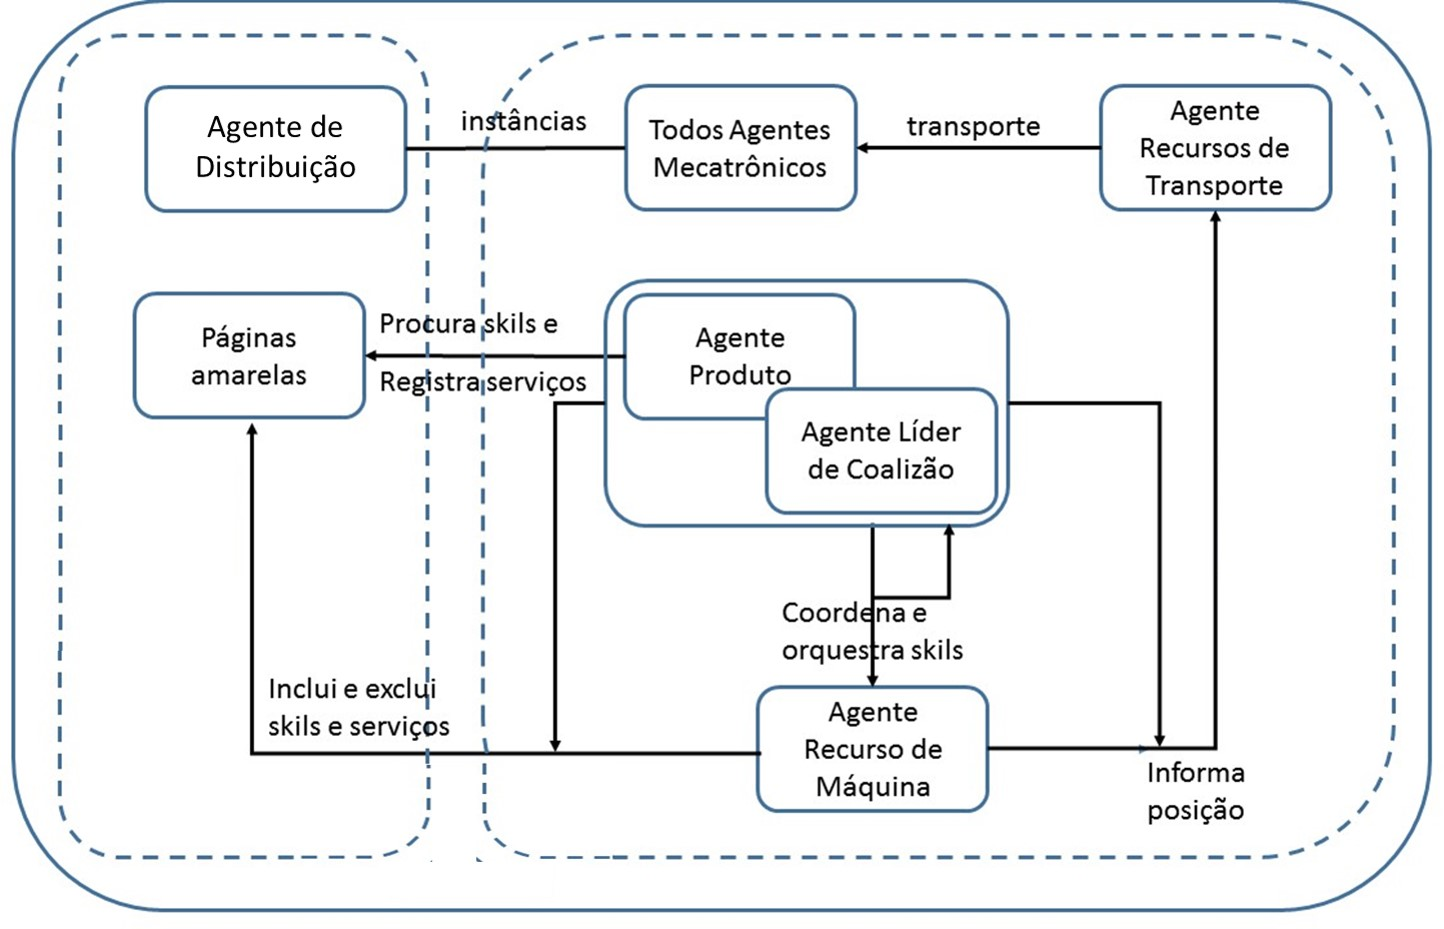
\includegraphics[width=0.8\textwidth]{img/F8_1_SIAPE_Arquitetura_EPS.jpg}
	\caption{IADE: Arquitetura de referência EPS}
	\label{fig:arq_referencia_eps}
	{\footnotesize{Fonte: \cite{CAVALCANTE2012a}}}
\end{figure}

Sua arquitetura de referência pode ser vista na Figura~\ref{fig:arq_referencia_eps}, que mostra dois tipos de agentes mecatrônicos: agente de recurso e agente de coalizão. Agentes de produtos são um tipo de agente de coalizão. Agentes de transporte são um tipo de agente mecatrônico normal, mas especializado no sistema de transporte.

Tais sistemas estão sendo desenvolvidos e testados objetivando as fábricas inteligentes e a padronização proposta pela Plataforma~\cite{VDE2014} da Indústria 4.0 ~\cite{DRATH2014}. 

Historicamente, EPS é a abordagem mais nova de um movimento que começa a partir da década de 80. A Figura~\ref{fig:evolucao_paradigmas} ilustra a evolução dos paradigmas de produção, mostrando também os nomes dos pesquisadores que iniciaram aquele paradigma.

\begin{figure}[b]
	\centering
	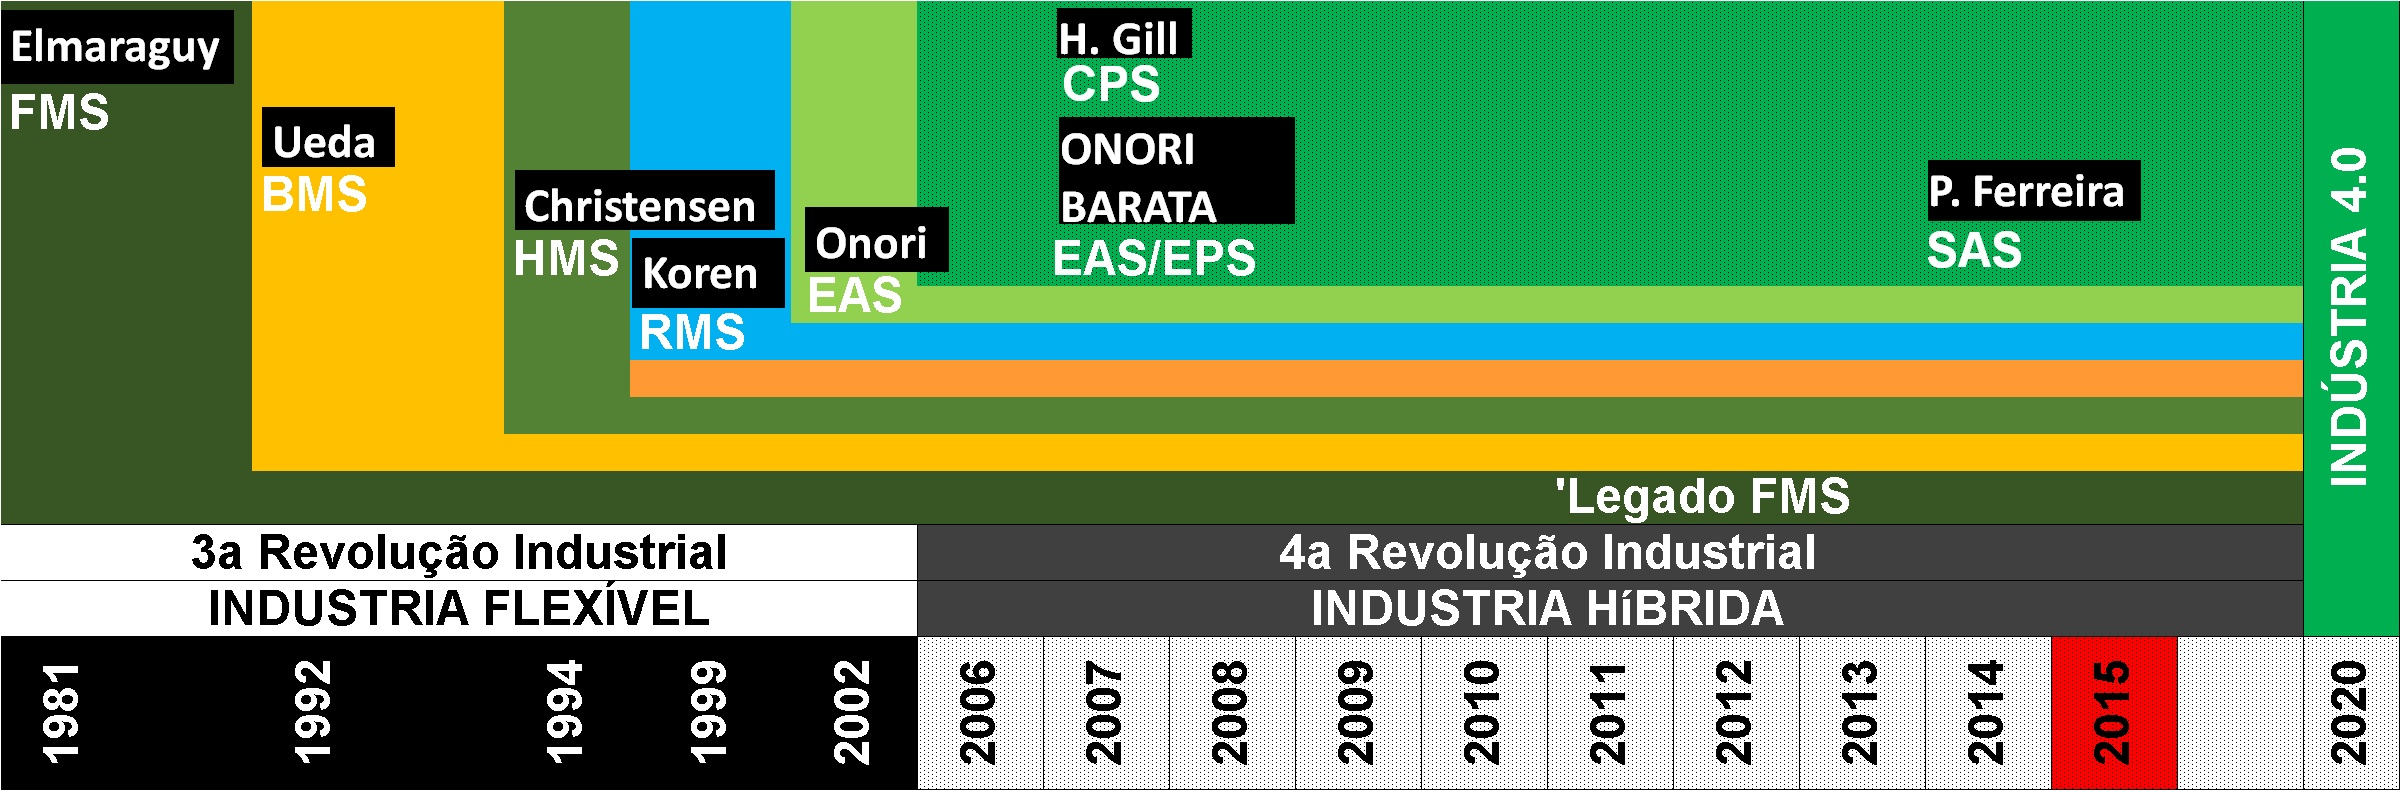
\includegraphics[width=\textwidth]{img/F8_2_SIAPE_PARADIGMAS.jpg}
	\caption{Evolução do Paradigmas de Produção}
	%\footnotesize{Fonte: O autor}
	\label{fig:evolucao_paradigmas}
\end{figure}

Os EPS possuem algumas características interessantes, pois possuem em um grau elevado, adaptabilidade, evolutibilidade, modularidade e sua granularidade pode ser ajustada conforme a complexidade do sistema. Para este trabalho, estes termos tem os seguintes significados:

\textbf{Adaptabilidade} -- o sistema tem de ser capaz de propor uma configuração alternativa para minimizar os efeitos adversos de perturbações. Adaptação é de curto prazo e, normalmente, implica \textit{auto-reconfiguração} na forma de ajustes de parâmetros~\cite{ROSA2013c}.

\textbf{Evolutibilidade} -- 
Em relação à \textit{evolução}, o sistema tem de ser capaz de permitir a introdução ou remoção de módulos existentes sem implicar na performance e no funcionamento do sistema. Assim, o sistema evolui a medida que novos produtos são colocados em produção, isto é, conforme o ambiente industrial modifica-se no tempo. A evolução se caracteriza num processo de longo prazo, podendo o sistema evoluir até o limite da tecnologia ou ao limite da planta fabril~\cite{ROSA2013c}.

\textbf{Modularidade} -- denotada pela noção de independência entre os módulos dos sistema.

\textbf{Plugabilidade} -- se o sistema pode inserir ou remover módulos como parte de seu funcionamento normal em tempo de produção.

\textbf{Granularidade} -- que evidencia o quanto de informação um agente deve possuir sobre os demais agentes, e a quantidade destes, a fim de se conseguir um objetivo definido.

Para este texto, \textbf{reconfigurabilidade} é a habilidade do sistema de redesenhar seu layout sem comprometer o funcionamento do sistema. Portanto, a plugabilidade é uma espécie de reconfigurabilidade. 

Quando um sistema possuir algum grau desses parâmetros, ele é dito possuir a \textbf{auto-organização} e o sistema é dito ser \textbf{dinâmico}.


\subsection{Visão geral da arquitetura EPS}

EPS é baseado em agentes inteligentes. Nas primeiras arquiteturas havia a definição de muitos tipos diferentes de agentes, capazes de tratar certos aspectos do sistema produtivo, tais como transporte, acesso hardware ou agentes de coalizão.

Simplificações tem sido propostas ao longo do tempo. Atualmente, EPS pode ser descrito como uma abordagem multiagente capaz de auto-organização e execução de processos complexos através da interação entre os agentes que formam o sistema. Há basicamente dois tipos de agentes em EPS: os agentes mecatrônicos e os agentes não mecatrônicos. Dentre os agentes mecatrônicos, pode-se citar a existência de dois subtipos: agentes cognitivos e agentes motores. 

Os agentes cognitivos são os responsáveis pela coalizão de outros agentes mecatrônicos: cognitivos ou motores. Os agentes motores são os que possuem acesso ao hardware elétrico e/ou mecânico do equipamento mecatrônico.

Os diversos tipos de funções no sistema produtivo são implementados por meio destes tipos de agentes. Por exemplo, um agente produto é um tipo especial de agente cognitivo que possui a inteligência de como montar a si mesmo através da coalizão dos agentes mecatrônicos (recursos/ferramentas) do sistema produtivo.

Agentes mecatrônicos possuem \textit{habilidades}, isto é, o que eles são capazes de fazer no sistema produtivo. Pode ser algo como \texttt{produzirProdutoA()} ou \texttt{baixarSugador()} ou ainda como \texttt{fecharGarra()}. \par 
Essas habilidade ou serviços que os agentes executam são chamados de \textit{skills}. \par 
Um agente mecatrônico pode possuir um ou mais \textit{skills}, que podem/são disponibilizados para todos os outros agentes do sistema.

Dentre os agentes não mecatrônicos cita-se: o agente intermediador (\textit{gateway}) que tem a função de interligar o sistema de produção EPS com outros sistemas legados e/ou interface homem máquina; e o agente de páginas amarelas (\textit{Yellow Page Agent} - YPA) que é o responsável pelo registro e busca de \textit{skills} por todo o sistema.

%=====================descrição da arquitetura EPS de Cavalcante=======================================================

\subsection{Descrição da Arquitetura EPS de Cavalcante }
 	 	  
A arquitetura \textit{EPS} proposta por Cavalcante denominada de Arquitetura Baseada em Agentes e Auto-Organizável Para a Manufatura  está ilustrada na Figura \ref{F132} e é descrita a seguir.

A arquitetura é formada por dois tipos de agentes:
 	 
 \textbf{O agente cognitivo} é o responsável pela lógica da aplicação empregada na situação e escolhe uma decisão a ser realizada, por outro agente cognitivo ou por um agente motor. A camada superior funciona como aplicação do agente e  a camada inferior funciona como interface de comunicação com os outros agentes do sistema, e promove a seleção e as requisições feitas para os outros agentes do sistema.
 	 	  
  \textbf{O agente motor} por sua vez, tem sua camada superior funcionando como comunicação e a camada inferior como a aplicação do agente. A camada superior recebe a comunicação das operações a serem realizadas que são enviadas pelo agente cognitivo. A camada inferior além de ter a função da aplicação do agente, funciona como camada de sensoriamento percebendo o ambiente e informando as condições sentidas ao agente cognitivo, para que este tome as decisões necessárias e as realize as tarefas atribuídas ao sistema.
 	 	  
  	 	  \begin{figure}
  	 	  	\centering
  	 	  	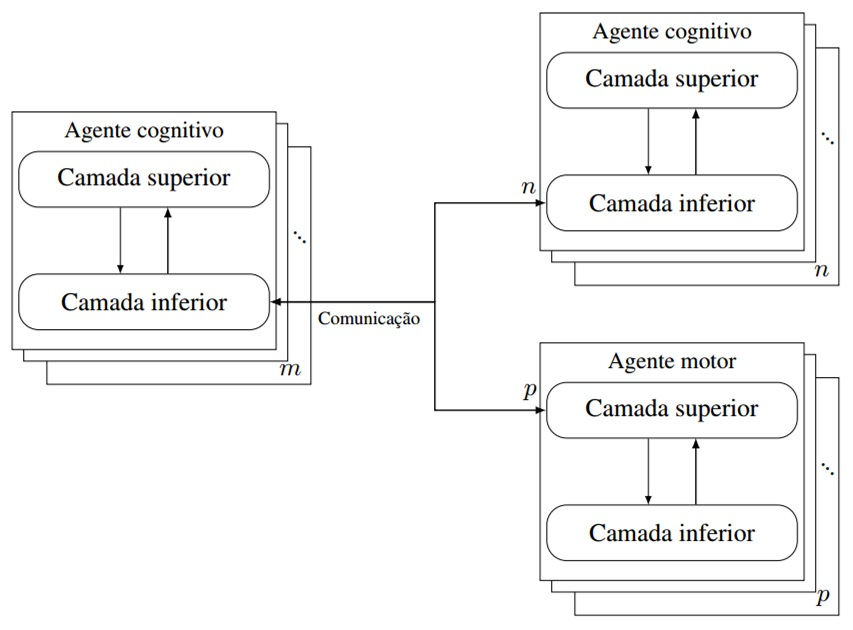
\includegraphics[width=12cm, height=7cm]{F132_ARQUITETURA_BAAOPM.jpg} 
  	 	  	\caption{Visão geral da Arquitetura proposta por Cavalcante}
  	 	  	\footnotesize{Fonte: \cite{CAVALCANTE2012a}}
  	 	  	\label{F132}
  	 	  \end{figure}
  	 	  
 	 	  \begin{figure}[b]
 	 	  	\centering
 	 	  	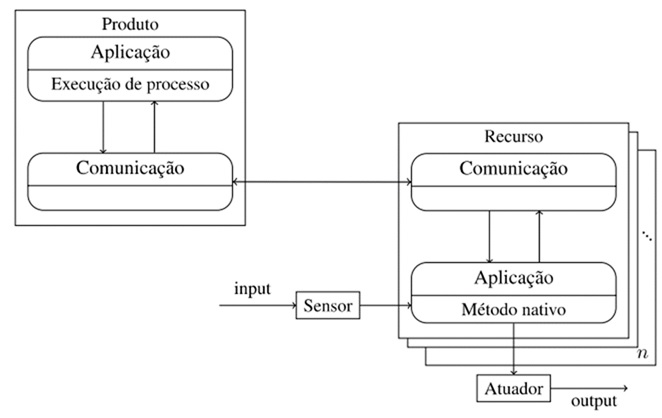
\includegraphics[width=12cm, height=6cm]{F133_ARQUITETURA_BAAOPM_MONTAGEM.jpg} 
 	 	  	\caption{Arquitetura para uma aplicação em um sistema de montagem}
 	 	  	\footnotesize{Fonte: \cite{CAVALCANTE2012a}}
 	 	  	\label{F133}
 	 	  \end{figure}	
 	 	  
 A arquitetura foi dividida para uso em dois tipos de aplicações: em sistemas de montagem e em sistemas de controle. A aplicação para um sistema de montagem é formado por agentes cognitivos, que modelam os produtos a serem montados, e por agentes motores, que modelam os recursos de hardware que realizam operações no processo de montagem. A Figura \ref{F133} ilustra a aplicação desta arquitetura para sistemas de produção. Nesta pode-se identificar o agente produto que é modelado por agentes cognitivos, e agentes motores que modelam os recursos de produção. 
 	 	  
 	 	  
 Já a Figura \ref{F138} ilustra a implementação de referência de EPS conforme o projeto \textit{IDEAS}. Os agentes desta implementação são assim chamados:
 	 	  
 	 	  \begin{description}	
 	 	  	
 	 	  	\item[\textit{DeploymentAgent (DA)}]  representa o agente de distribuição, isto é, o agente que  pesquisa serviços de páginas amarelas, os \textit{skills} que devem ser trocados entre agentes para negociação até que se atinja os objetivos propostos pelo sistema. O \textit{DA} também permite que o sistema seja configurado através de ferramentas externas.
 	 	  	
 	 	  	\item[\textit{YellowPageAgent (YPA)}] Agente Páginas Amarelas - é o responsável por registrar as habilidades dos agentes que não são mecatrônicos. Ele fornece uma infra-estrutura que permite que outros agentes registrem suas informações e que estas sejam consultadas por outros agentes que estejam necessitando de determinado \textit{skil}.
 	 	  	
 	 	  	\item[\textit{Resource Agente (RA)}] são os agentes que externam funcionalidades ao sistema de montagem. Este é o agente básico da biblioteca \textit{IADE} que controla os módulos de hardware que podem ser conectados ou desconectado no hardware do sistema, isto é, este agente é dotado de skills atômicos que são diretamente relacionado com o hardware. Este fato proporciona  ao sistema a capacidade de reconfiguração de funcionalidades no nível do controlador. 
 	 	  	
 	 	  	\item[\textit{Coalition Leader Agent (CLA)}]  são agregadores e a base da reutilização de funcionalidades em qualquer nível. É o agente que suporta a composição de competências. Isto significa que o \textit{CLA} é capaz de reagir às perturbações no ambiente, tais como a adição ou remoção de funcionalidades e falhas sob o seu domínio. 
 	 	  	
 	 	  	\item[\textit{Transport Agent (TA)}] são abstrações do sistema de transporte, isto é, é o agente que abstrai as entidades de transporte por exemplo, transportadores ou \textit{AGV}. É responsável pela computação do custo de transporte entre localizações no sistema.
 	 	  	
 	 	  \end{description}	
 	 	  
 	 	  Considerando a nomenclatura de Cavalcante, os \textit{CLAs e PAs} são agentes cognitivos e \textit{RAs e TSAs} são agentes motores.
 	 	  
 	 	  \begin{figure}
 	 	  	\centering
 	 	  	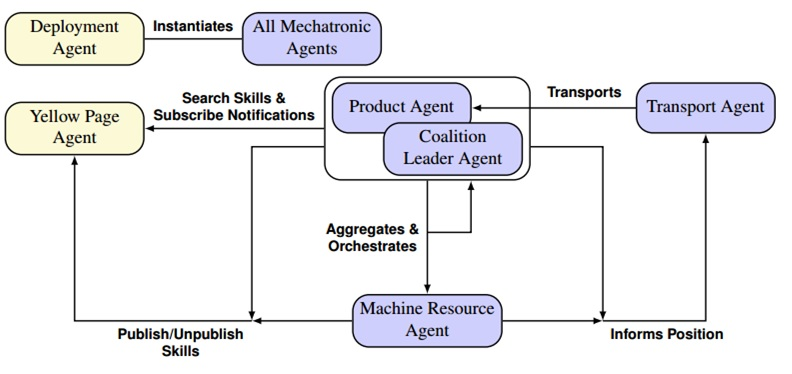
\includegraphics[width=12cm, height=6cm]{F138_IADE_cavalcante.jpg} 
 	 	  	\caption{Implementação de referência EPS}
 	 	  	\footnotesize{Fonte: \cite{CAVALCANTE2012a}}
 	 	  	\label{F138}
 	 	  \end{figure}	 


%===============================================================================================================
  \subsection{A Arquitetura do SIAPE}

%=================================================================================================================

A Figura \ref{fig:eps_arquitetura_1} ilustra a arquitetura do SIAPE que foi baseada na arquitetura de Cavalcante para um sistema de montagem. Na figura os recursos são agentes cognitivos ou agentes motores que realizam as operações do processo de montagem diretamente nos sensores e atuadores do sistema. O agente motor principal, no SIAPE, recebe o nome de AcHw. Assim como todos os módulos e agentes do SIAPE, o AcHw foi concebido a partir da aplicação do Método de Desenvolvimento de Sistemas Evolutivos (MeDSE), aplicado ao desenvolvimento do SIAPE. O método de desenvolvimento é detalhado no Capítulo 3.

O agente AcHw do SIAPE  tem a principal função de identificar, em tempo real, os módulos que estão presentes no  sistema e informá-los ao agente  \textit{YPA}. Uma vez identificados no \textit{YPA}, os demais agentes tem acesso aos \textit{skills} do AcHW, notadamente o agente Anagram, que usa essas informações para realizar o processo produtivo. 

O agente \textit{OrderAgent} instancia agentes Anagram (agente Produto na arquitetura) que conhece todas as etapas de produção que envolve o agente Stamper e o agente Conveyor. 

O operador pode se comunicar com o sistema por meio da Interface Homem Máquina (IHM) que acessa diretamente o \textit{OrderAgent}. Este também pode ser usado com a função de \textit{gateway} na comunicação tanto de sistema \iQuatroZero, isto é, sistemas aderentes à plataforma \iQuatroZero, quanto de ambientes \iTresZero, isto é, sistema flexíveis comuns aos sistemas da 3ª Revolução Industrial.

Resumindo, na aplicação de tal arquitetura neste trabalho, tem-se os seguintes agentes:

\begin{itemize}
	\item YPA - registro e busca de \textit{skills}
	
	\item OrderAgent - um \textit{gateway} para a interface homem máquina do EPS; instancia os anagramas de acordo com a ordem de serviço gerada na IHM.
	
	\item Anagram - um agente cognitivo que representa um produto a ser produzido.
	
	\item AcHw - um agente motor responsável pelo acesso ao hardware eletrônico do sistema.
	
	\item Conveyor - um agente cognitivo que representa a esteira do sistema; esconde do agente produto a complexidade do acesso ao hardware para se realizar o transporte.
	
	\item Stamper - um agente cognitivo que representa um módulo carimbador do sistema; esconde do agente produto a complexidade do acesso ao hardware para se carimbar letras do anagrama na palete.
\end{itemize}


\begin{figure}
	\centering
	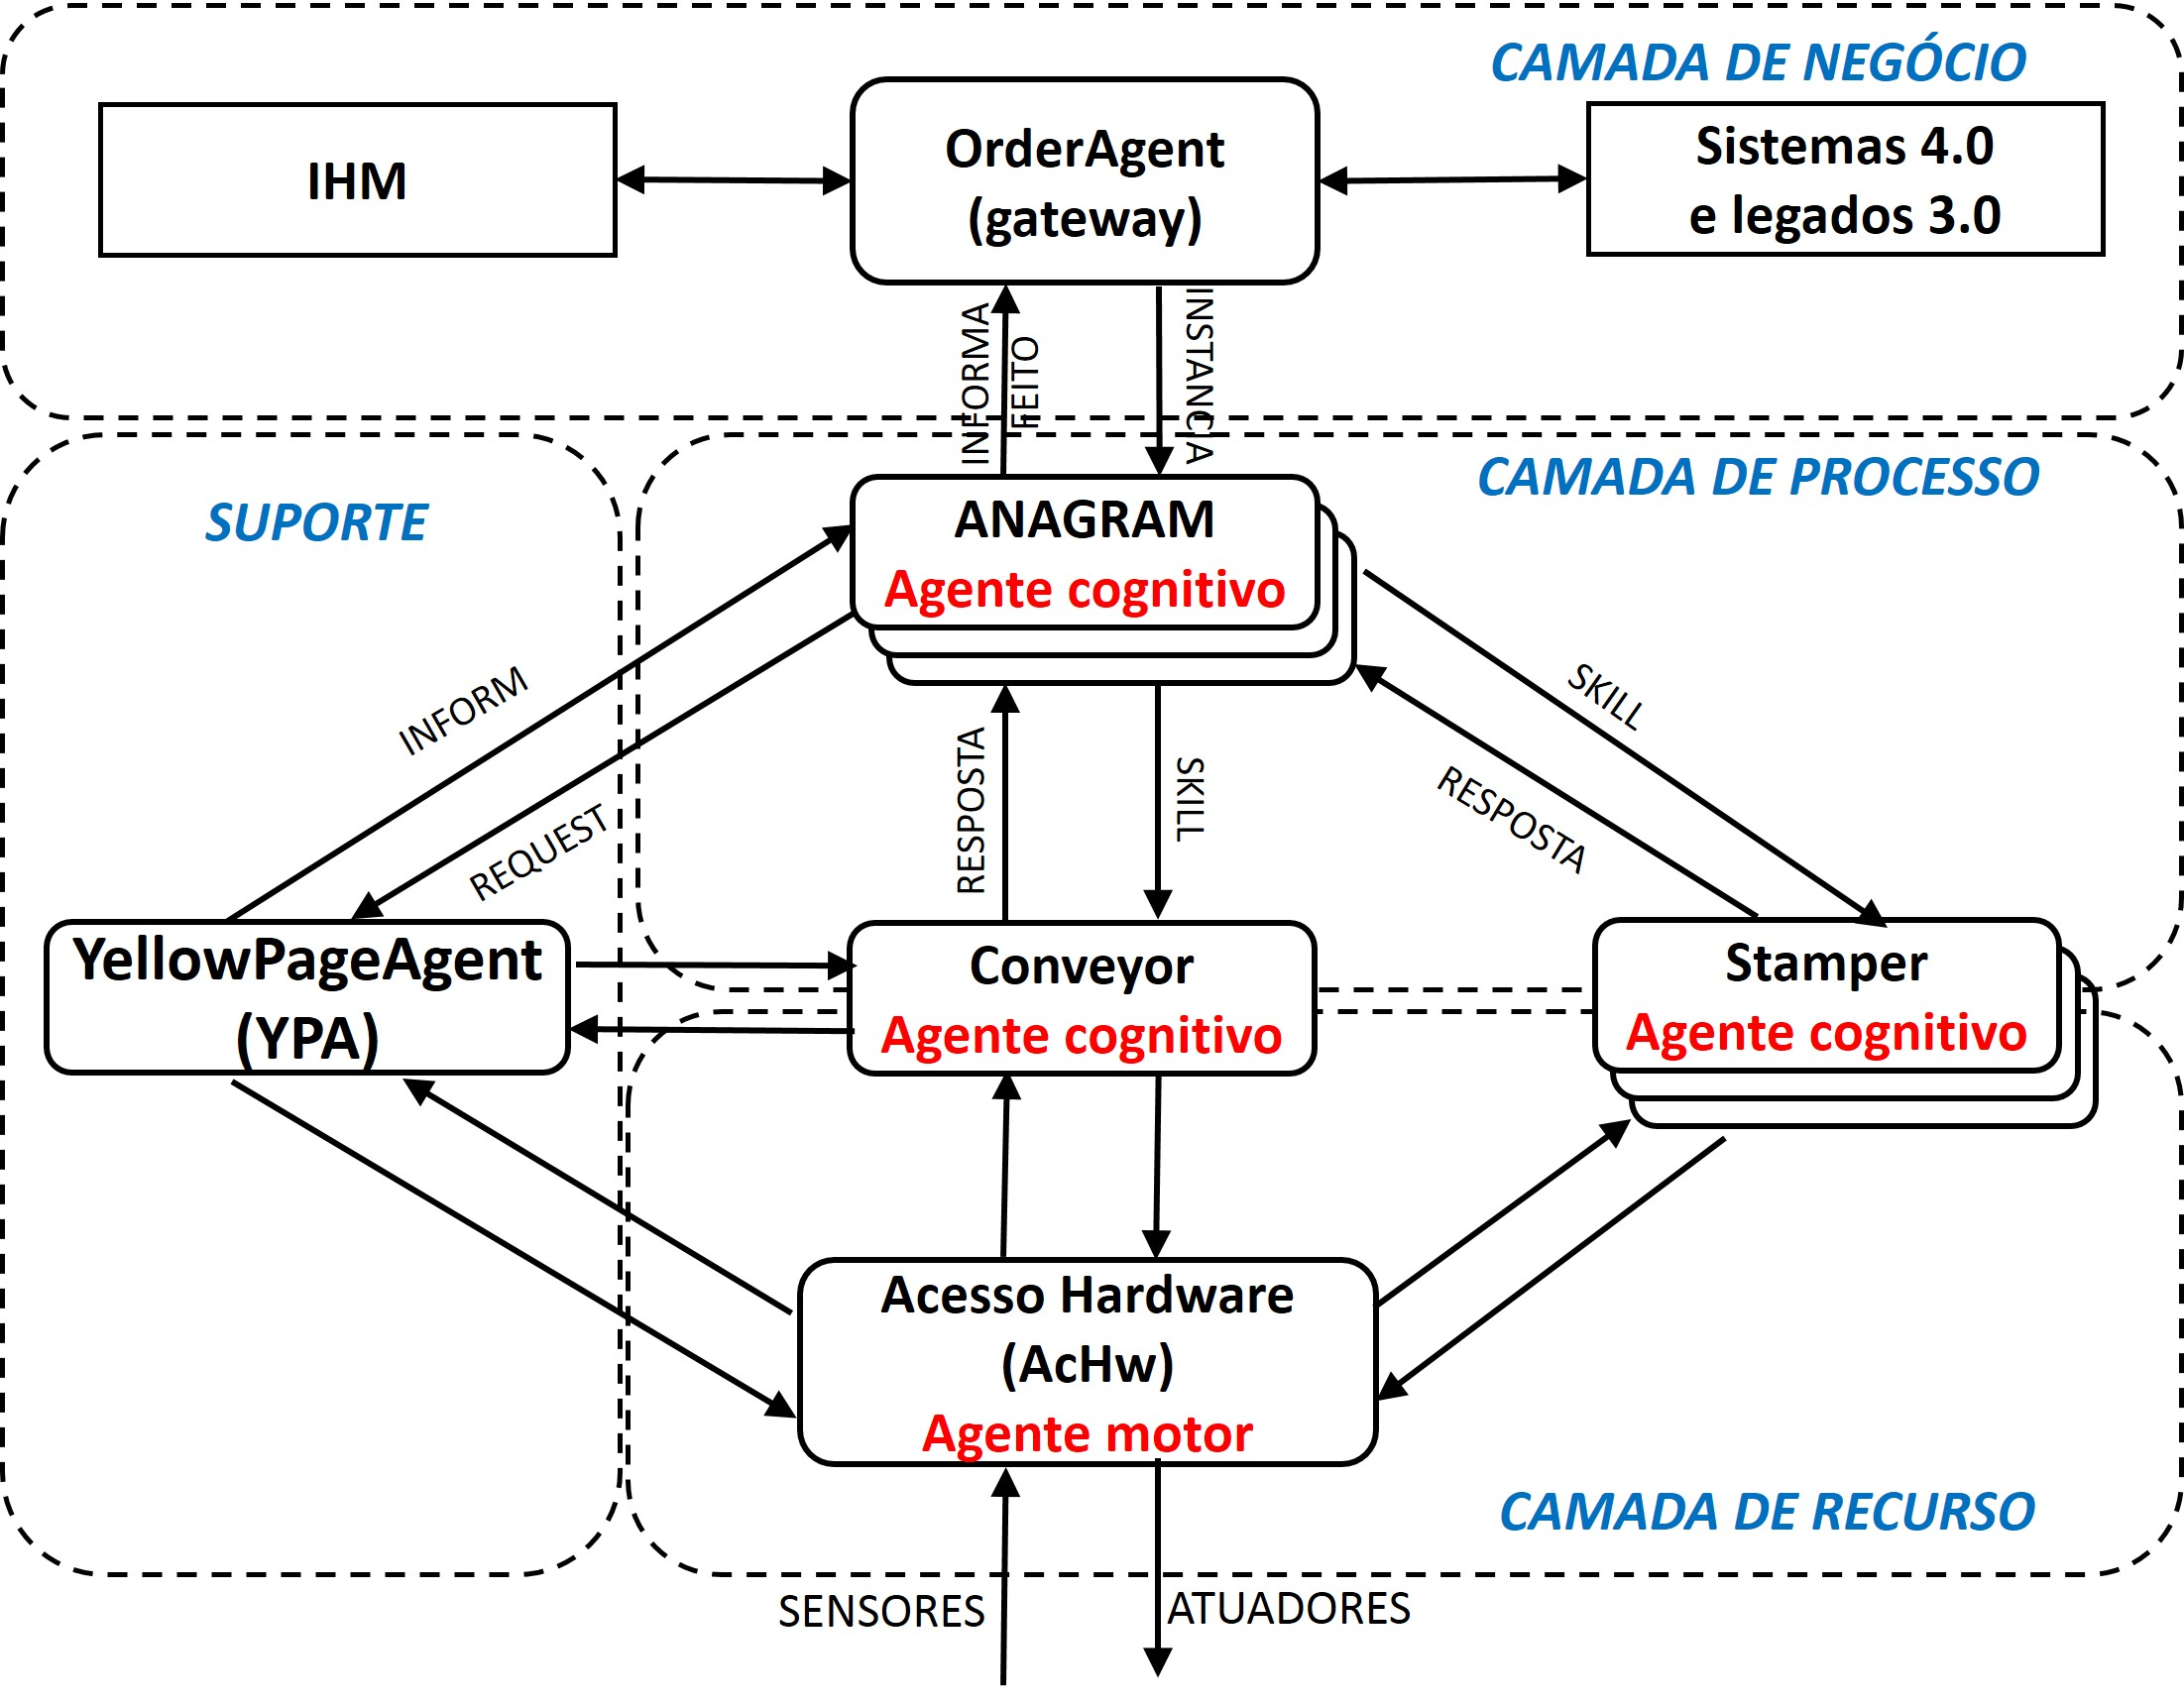
\includegraphics[width=0.8\textwidth ]{img/F140_SIAPE.jpg}
	\caption{Aplicação da arquitetura EPS no SIAPE}
	%\footnotesize{Fonte: O autor}
	\label{fig:eps_arquitetura_1}
\end{figure}

A principal contribuição do SIAPE  à arquitetura de Cavalcante é o reconhecimento da existência do agente \textit{OrderAgent}, na camanda de negócios, que é um tipo de agente que permite a comunicação externa com os agentes internos ao sistema, contudo não pode ser enquadrado como um agente cognitivo ou motor da arquitetura. A diferença reside no fato da função \textit{gateway} do agente de ordem de serviço permitir a comunicação com o operador, através da IHM, de uma forma transparente.

O agente Produto e o agente Recurso da arquitetura SIAPE, funcionam conceitualmente exatamente igual à arquitetura de Cavalcante, isto é, o agente cognitivo responsável pela lógica e inteligência do sistema e o agente motor fica responsável por receber as decisões do agente cognitivo e realizar as operações necessárias no processo produtivo.


%===================================================================

\section{Conceituação teórica de termos importantes para a pesquisa}	

O avanço da fronteira da ciência aproxima cada vez mais as áreas da Engenharia e da Computação. Neste contexto encontramos antigos termos combinados entre si para criar novos significados. O objetivo dessa seção é esclarecer o significado de alguns destes termos que são utilizados na sequência deste trabalho e evitar erros em suas interpretações.



\subsubsection{Auto-organização e emergência}

Sistemas EPS são dito auto-organizáveis e emergentes. 

Um sistema é chamado de auto-organizado quando é capaz de mudar a sua organização interna autonomamente, isto é, sem interferências externas, a fim de responder a uma mudança ambiental relevante. A \textbf{auto-organização} é, pois, a propriedade de um sistema de adquirir uma estrutura espacial, temporal ou funcional sem interferência externa. 

Há várias formas de se fazer tal auto-organização, por exemplo, através de um subsistema que detém toda a informação necessária para realizar a configuração do macro-sistema mediante uma análise cuidadosa do ambiente e das perturbações sofridas; esta é a solução centralizada. No entanto, quando o sistema não tem essa entidade centralizadora, pode ainda ser capaz de auto-organização quando os elementos que formam o sistema forem suficientemente inteligentes para se perceberem, interagirem e montarem a topologia mais adequada para a execução de um objetivo (ou múltiplos objetivos). Quando isto ocorre, é dito que o sistema é \textbf{emergente}, pois aparecem propriedades e padrões no nível macro, mas a informação de como tais padrões e propriedade devem ser formados não estão descritas \textit{claramente} nos elementos que formam o sistema. Diz-se que tais propriedades emergem da interação dos elementos constituintes do sistema. Do ponto de vista micro, as ações dos agentes são aleatórias, mas resultam em uma propriedade emergente no nível macro.

Um EPS possui auto-organização porque é capaz de autonomamente ajustar-se a variações na demanda, bem como reconhecer os elementos que o forma. Também é dito que possui \textbf{emergência} porque as interações entre os agentes ocorrem de forma dinâmica (não prevista), entretanto, um produto final é montado.

O período atual está sendo marcado pela busca de soluções para o problema recorrente da customização em massa. Esse período é, neste estudo, denominado de Indústria Híbrida devido ao fato da convergência de paradigmas, sistemas, arquiteturas e ferramentas na busca de uma solução ótima para o fenômeno da customização, sem no entanto se chegar a um denominador comum. 

Os sistemas evolutivos, com a aplicação de algumas de suas capacidades e propriedades, nesse caso, auto-organização e emergência, apontam para soluções eficazes, vencidas as complexidades, na busca de soluções definitivas para o problema recorrente da customização de massa.



\subsection{Plataforma da Indústria 4.0}	

O \textit{white paper} da Indústria 4.0~\cite{BITKOM2015} formulou as questões centrais da \iQuatroZero, a partir de um ponto de vista da pesquisa e inovação. Das recomendações publicadas, quatro são consideradas e descritas neste trabalho, conforme segue:

\begin{description}
	\item[A integração vertical (IVe)] -	
	é caracterizada pela capacidade dos sistemas integrarem os seus processos técnicos aos processos de negócio da empresa, para auxiliar no processo de decisão estratégica empresarial; uma das propriedades relacionadas é a interoperabilidade entre os sistemas; 
	
	\item[A integração horizontal (IHo)] -
	é a agregação, em tempo real~\cite{VDE2014} dos elementos de conhecimento que tais sistemas geram no chão--de--fábrica. Para isso relaciona-se a comunicação, o planejamento e a programação de tais sistemas, contendo elementos que serão usados para incorporar raciocínio baseado em casos de uso, evidenciando a capacidade de evoluir com a mudança dos requisitos de produção; 
	
	\item[A integração humana (IHu)] -
	é caracterizada pelo uso das capacidades de criação dos seres humanos considerados no desenvolvimento dos sistemas e na recuperação dos sistemas legados \iTresZero;
	
	\item[A engenharia 4.0 (E4.0)]
	é denotada pelos domínios dos conhecimentos de Engenharia durante todo o processo do ciclo de vida do produto, os quais o projetista deverá capturar com base na especificação do produto, desde a concepção ao encerramento do projeto, levando-se em conta as tarefas e habilidade dos agentes mecatrônicos do sistema. Inclui--se aqui o domínio da eletrônica, da mecânica, de software, das redes, entre outros;
\end{description}
	
A Indústria 4.0 representa a situação futura, entretanto, na atualidade, já estão sendo produzida as condições necessária ao seu funcionamento, a saber: os ciberespaços, contendo as ciberestruturas~\cite{NITRDGROUPS2010} os dispositivos e tecnologias que serão utilizados pela Indústria 4.0, que por sua vez, são baseados nos paradigmas evolutivos e nos (CPS)~\cite{LEE2008}. 

%Nesse contexto, a \textit{Internet of Things}~(IoT)~\cite{ROTONDI2013b} será obrigatória, e os grandes centros de tecnologias estarão, finalmente conectadas e interagindo entre os centros de referências de Ciência, Tecnologia e Inovação em torno do globo terrestre. 

Neste contexto, os grandes centros de desenvolvimento de C\&T\&I estão tomando iniciativas que visam a implantação da \iQuatroZero. Por exemplo, o Horizon 2020~\cite{H2020} é o maior Programa de Investigação e Inovação da UE. O programa já conta com cerca de 80 bilhões de euros em financiamento disponível ao longo de 7 anos (2014-2020), além do investimento privado que esse dinheiro vai atrair. Ele promete mais avanços, descobertas e estreias mundiais, possibilitando grandes ideias saírem do laboratório para o mercado. Visto como um meio de impulsionar o crescimento econômico e criar empregos na UE tem o apoio político dos líderes europeus e dos deputados do Parlamento Europeu. 
%Eles concordaram que a pesquisa é um investimento no futuro para o crescimento, o emprego inteligente, sustentável e inclusivo. 
	
%Quando a constante utilização de sistemas \textit{FMS} como solução para os lotes médios já não tinha a mesma eficácia, a personalização de produtos passou a ser tratado pela agilidade. Para isso os sistemas baseados em \textit{ FMS} foram substituídos pelos sistemas baseados nos paradigmas \textit{BMS, HMS e RMS}. No final desse período a agilidade teve sua eficácia reduzida como solução para o fenômeno da customização em massa e surge os sistemas emergentes baseados nos paradigmas \textit{EAS/EPS} e a auto-organização. \textit{A emergência aqui entendida como a propriedade de um sistema ser construído de forma determinística, por meio dos conceitos da auto-organização. A auto-organização, por sua vez é a propriedade de um sistema de adquirir uma estrutura espacial, temporal ou funcional sem interferência externa.}\par
	

\subsection{Termos do Sistema de Produção}	

No jargão do ambiente industrial, aparecem alguns termos que igualmente precisam ser aclarados. Neste trabalho, os seguintes termos terão os subsequentes significados:

%=====================================================================
\begin{figure*}
	\centering
	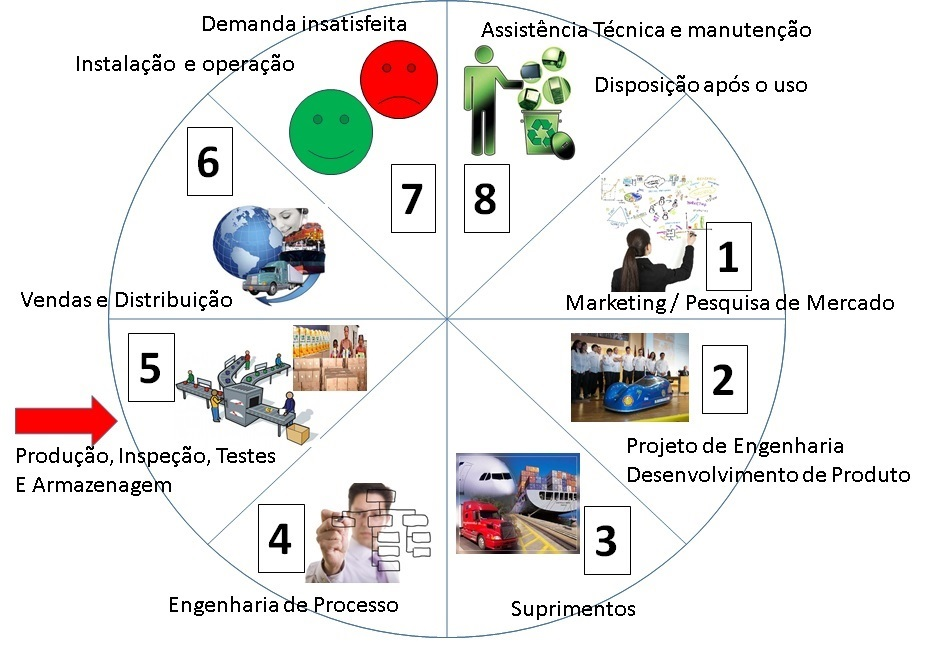
\includegraphics[width=0.8\textwidth]{img/F6_SIAPE_Ciclo_de_vida_do_Produto.jpg} 
	\caption{SIAPE: Ciclo de vida do produto}
	\label{F6}
\end{figure*}
%======================================================================
	
\begin{description}
	\item[Ciclo de vida do produto] -
	O ciclo de vida do produto descreve as fases do produto desde o seu nascimento até o seu descarte na sociedade. Tal ciclo é mostrado na Figura~\ref{F6}. Analisando a figura, tem-se o ciclo iniciado na fase 1, onde a equipe de marketing realiza pesquisas no mercado de demandas não atendidas (fase 7) para que esforços sejam aplicados nessa direção; na fase 2, a necessidade não atendida é transformada num produto a ser produzido; a fase 3, ilustra a compra e a logística dos insumos necessários para a realização do produto; na fase 4, a Engenharia de Processo prepara o produto para produzido em linhas de produção; a fase 5 acontece nas linhas de produção propriamente ditas, onde são efetivamente montados os produtos; na fase 6 o produto é vendido e distribuídos no comércio; a fase 7 ilustra o atendimento da demanda insatisfeita através do atendimento às necessidades do cliente; Na fase 8 tem-se a assistência técnica e a o posterior descarte após o uso do produto finalizado.
	
	\item[Reconfiguração ou tempo de \textit{setup} de linha de produção]
	Tempo de \textit{setup} é o período em que a produção é interrompida para que os equipamentos da linha de produção sejam ajustados, configurados ou reconfigurados. O tempo de setup está diretamente relacionado com as variações do produto e o planejamento da produção realizado pela indústria.
	Nos sistemas de produção em lotes, as paradas para ajustes estão mais presentes devido à necessidade de se produzir uma grande variedade de produtos, tornando o controle deste período uma necessidade crítica, fundamental para a garantia de uma boa produtividade. 
	
	\item[Configuração ou \textit{lead time} de linha de produção]
	É o tempo decorrido desde a concepção do produto até a montagem da linha e sua efetiva entrada em produção com toda a capacidade produtiva.
	
	\item[Curva de crescimento ou \textit{ramp up} de linha de produção]
	\textit{Ramp up} é um termo usado em economia e negócios para descrever um aumento firme na produção. Neste trabalho de pesquisa este termo está restrito à linha de produção.  Quando um plano de produção de um novo produto entra em linha, os recursos não conseguem atingir a quantidade ideal planejada e ajustes são realizados para que essas quantidades sejam alcançadas. O período entre o início da produção até que os recursos produtivos consigam atingir a quantidade planejada é definido como o \textit{ramp up}.
\end{description}

	
\begin{figure}[h!]
	\centering
	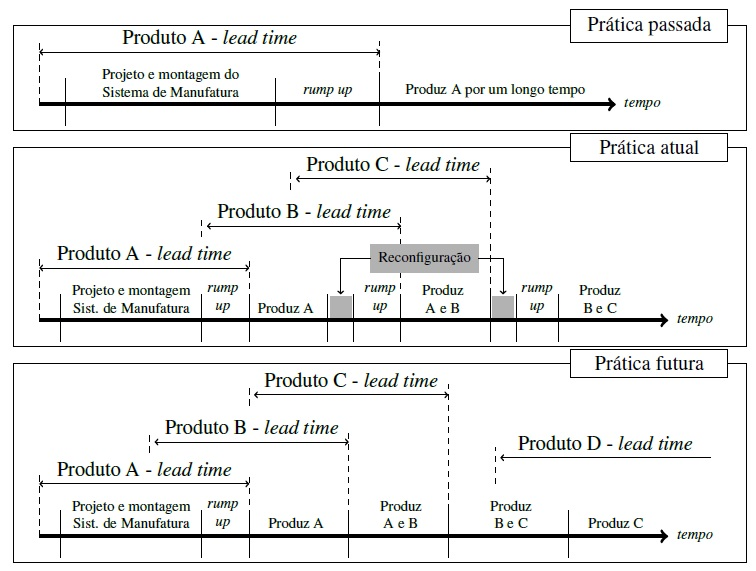
\includegraphics[width=\textwidth, height=10cm]{img/F8_SIAPE_Lead_Time_EPS.jpg} 
	\caption{Redução do Lead time de Produção}
	{\footnotesize{Fonte: \cite{KOREN1999} com adaptações de \cite{CAVALCANTE2012a}}}
	\label{F8}
\end{figure}
	

Com os volumes altos de produção, as configurações entre produtos eram realizadas em espaços de tempos que não preocupava o setor produtivo, entretanto tal não é mais a realidade atual. A Figura~\ref{F8} descreve esse processo onde pode ser evidenciado que o produto A, na prática passada de manufatura, produz durante um longo período de tempo, enquanto que atualmente, convivem vários produtos (A,B,C) simultaneamente em produção. Mais ainda, vislumbra-se que a prática futura exija que um tempo de reconfiguração e as paradas de linha tendam a zero.




\subsection{Agentes e Sistemas Multi-Agentes (MAS)}	

O termo \textbf{agente} continua sem uma definição universalmente aceita, existindo  ainda muito debate e controvérsias, contudo para nortear este trabalho, o termo agente foi conceituado como uma entidade abstrata que age no mundo real por meio de sensores que percebem o ambiente e atuadores que alteram esse ambiente para atingir metas estabelecidas. Esse conceito tem suas bases nas seguintes definições:\par 

\begin{quote}
	\textit{``Um agente é algo capaz de perceber seu ambiente por meio de sensores e de agir sobre esse ambiente por meio de atuadores''} \cite{Russell_Norvig1995}.
\end{quote}

\begin{quote}
	\textit{``Um agente é um sistema de computador que está situada em algum meio, e que é capaz de agir autonomamente neste ambiente, a fim de atender seus objetivos de projeto''} \cite{WOOLDRIDGE2002,WOOLDRIDGE2007}
\end{quote}

Agentes conseguem perceber o ambiente e agir sobre ele para alterá-lo. Dentre as diversas características de agentes, neste trabalho foram enfatizadas as seguintes: 

\begin{enumerate}
	\item Autonomia - agentes atuam cumprindo seus objetivos individuais; 
	
	\item Sociabilidade - agentes interagem entre si estabelecimento uma sociedade de agentes; 
	
	\item Racionalidade - um agente pode raciocinar sobre os dados que ele recebe, através de seus sensores ou de comunicação com outros agentes, a fim de encontrar a melhor solução para atingir o seu objetivo; 
	
	\item Reatividade - um agente pode reagir à mudanças no seu meio ambiente; 
	
	\item Pró-atividade - um agente pode ativamente agir no seu meio buscando os seus objetivos;
	
	\item Adaptabilidade - um agente é capaz de aprender e mudar seu comportamento quando uma solução melhor é descoberta. 
\end{enumerate}

Um sistema formado por agentes de diferentes tipos, ou vários agentes de um único tipo, que interagem entre si, formam um sistema multiagente (MAS). Tais sistemas são por natureza descentralizados e modulares, facilmente adaptáveis ao meio e capazes de resolver problemas complexos. 

Agentes são particularmente interessantes para os paradigmas industriais emergentes, pois estes são modulares, descentralizados, e necessitam de adaptação. Utilizando-se MAS nos sistemas evolutivos implica num ambiente de resiliência, sustentabilidade, robustez, tolerância a faltas~\cite{RIBEIRO2013a}. EPS é baseado em agentes. 

\subsection{O protocolo \textit{FIPA -- Foundation for Intelligent Physical Agents}}	

A \textit{FIPA (Foundation for Intelligent Physical Agents)} é uma associação internacional de companhias e organizações que juntas unem esforços a fim de produzir especificações para tecnologias de agentes que sejam aceitas de uma forma genérica. A FIPA promove um conjunto de tecnologias para diferentes áreas através de um conjunto de documentos que  definiram as regras que permitem a uma sociedade de agente existir, operar e ser gerenciada.  Dentre esses documentos encontram-se as especificações \textit{FIPA--ACL (Agent Communication Language)} que definem a comunicação entre os agentes. 

A Figura \ref{F93} ilustra os protocolos responsáveis pelo mecanismo de negociação e execução de funcionalidades dentro dos protocolos. A parte \textit{a} da figura mostra o Protocolo \textit{FIPA Request Interation Protocol} e a parte \textit{b} mostra o FIPA Contract Net Interation Protocol. Para este trabalho, o \textit{FIPA Request Interation Protocol} atinge os objetivos almejados.

Dentre os campos constantes nos campo definidos nas mensagens FIPA, os seguintes campos podem ser encontrados: 1) A Identificação do agente no sistema (AID); 2) O Conteúdo das mensagens expressas por caracteres; 3) O controle de mensagens, expresso pela identificação da conversa, o tipo de mensagem, tempo máximo, entre outros; 4)Ontologia, responsável pelo significado dos termos dentro do contexto de trocas das mensagens.


\begin{figure}
	\centering
	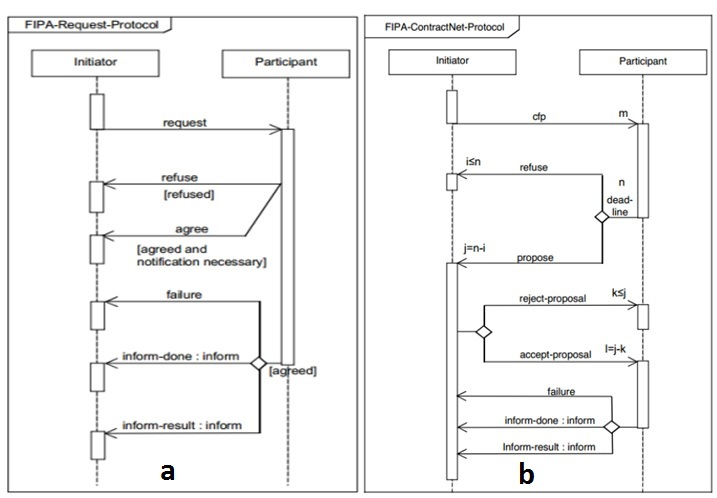
\includegraphics[width=16cm, height=10cm]{F93_SIAPE_FIPA.jpg}
	\caption{SIAPE: FIPA -- ACL}
	\footnotesize{Fonte:~\cite{FIPA2002b,FIPA2002c}}
	\label{F93}
\end{figure}		


\section{As Fases do Paradigma Evolutivo: acadêmica, experimental e holística}

Na Figura~\ref{F11} visualiza-se onde EPS está colocado, em termos históricos, no conjunto dos paradigmas da manufatura. Para uma análise específica das pesquisas realizadas em EPS, dividiu-se estes estudos em três fases distintas, a saber:


%==============================================================
\begin{figure*}[h]
	\centering
	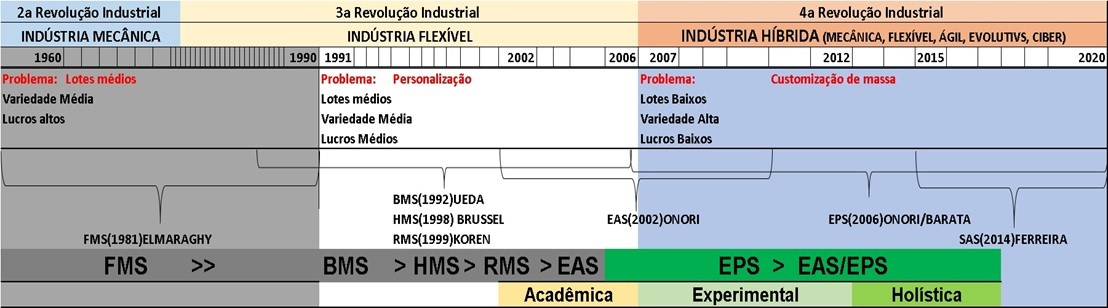
\includegraphics[width=\textwidth, height=6cm]{img/F11_SIAPE_Fases_EPS.jpg} 
	\caption{MeDSE - Fases do paradigma EPS}
	%\footnotesize{Fonte: Adaptado de~\cite{MUNZLINGER2012,MONTEBELO2000,SAMPAIO2007}}
	\label{F11}
	
\end{figure*}
%==============================================================

\begin{enumerate}
	\item A Fase Acadêmica: encontraram-se as pesquisas conceituais, simulações e primeiras provas de conceitos. Essa fase foi identificada entre os anos de 2002 quando surge a base dos sistemas evolutivos, o paradigma EAS e se estende até 2006 quando Onori estabelece as bases do paradigma \textit{EPS};
	
	\item  A Fase Experimental: onde o paradigma toma dimensões de testes e experimentos realizados por vários pesquisadores e dura até a prova de conceito do Projeto \textit{IDEAS} em 2012;
	
	\item  A Fase Holística: o paradigma percebe na prática a complexidade gerada pela interdisciplinariedade, e nesse momento, o foco foi além do chão-de-fábrica e transcendeu os campos Engenharia e da Computação para o campo da Economia, dos Sistemas complexos, da Inteligência Artificial, da Biologia e outros campos do conhecimento humano. 
\end{enumerate}


\subsection{A Fase Acadêmica do Paradigma Evolutivo}

Para encarar de frente o problema da personalização, foram criados os paradigmas \textit{BMS} utilizando seus \textit{modelons}, o \textit{HMS} com a ideia de \textit{holons} e o \textit{RMS} que, através da reconfiguração, consegue tratar as mudanças ambientais relevantes.

Na impossibilidade de solução ótima, pois cada tipo de sistema apresenta suas particularidades e desafios próprios, inicia-se a Fase Acadêmica do paradigma \textit{EPS}, no início do século XXI. Com o surgimento do paradigma \textit{EAS}, que utiliza das tecnologias de agentes e avanços no campo das linguagens de programação, modelagem e redes, \cite{ONORI2002} expandiram estes conceitos e os aplicaram na manufatura. EAS/EPS, usam módulos inteligentes, que comunicam-se em rede, através dos protocolos FIPA \cite{FIPA2013}, e princípios de Inteligência Artificial (IA) \cite{Russell_Norvig1995}. Realizam os conceitos da plugabilidade (\textit{plug and produce}) através da auto-organização e emergência de agentes.

O trabalho desenvolvido por \cite{BARATA2003} denotou uma arquitetura de referência para avaliar a questão da agilidade no chão de fábrica, e assim dominar as perturbações e incertezas do mercado que atingia o sistema. A composição do sistema e o seu comportamento são estabelecidas através da configuração das relações entre os módulos, usando mecanismos contratuais. A elevada capacidade de reutilização era motivada pelo conceito de módulos que eram facilmente atualizados para posterior reutilização. 

%As interações eram realizadas por módulos de fabricação e as coalizões regidas por contratos que eram configurados sempre que uma coalizão estivesse estabelecida. 



%=============================================================

\subsection{A Fase Experimental do Paradigma Evolutivo}

Em 2007 o trabalho conjunto de \cite{FREI2007} analisa o contexto e implicações do novo paradigma de produção \textit{EPS}.  Neste trabalho Frei reconhece a agilidade, a sustentabilidade e a reatividade como pontos chaves para tratar problemas de sistemas dinâmicos. Os sistemas evolutivos tendem para a solução do problema da customização, no entanto, precisam ser mais amadurecidos e tornados mais robustos para lidar com os distúrbios dos mercados atuais, e para isso, o paradigma \textit{EPS} tem sido evoluído e atualizado o suficiente para realizar essa tarefa.

O trabalho de \cite{MAFFEI2009} apresenta uma versão simplificada do paradigma \textit{EPS}, em uma forma de metodologia, que permitiu que o conceito de ciclo de vida de um produto e as ferramentas de avaliação de investimento puderam ser integrados. O trabalho identificou, entre outras coisas, as conquistas atuais dentro dos estudos do paradigma EPS que possibilitam às empresas relacionar requisitos de suas necessidade com algumas características de um modelo de negócio aplicável ao modelo atual de desenvolvimento de produto baseado em EPS.

\cite{CANDIDO2011} apresentaram a associação de \textit{EPS} com a abordagem \textit{Service Oriented Architectures} (SOA), na  busca de um objetivo comum, a nível do dispositivo para o domínio da automação industrial, delineando princípios arquitetônicos fundamentais e de um modelo de dispositivo para apoiá-lo. A associação entre SOA e EPS foi demonstrada através de um protótipo que confirmou a sua aplicabilidade num cenário esperado de caso de uso em automação industrial.

\cite{CAVALCANTE2012a} trazem uma visão geral dos paradigmas de manufatura, realiza uma breve descrição das pesquisas em torno do tema EPS e lança as bases para criação de uma linha de montagem que assimile os conceitos, tecnologias e paradigmas evolutivos que podem ajudar o Brasil nos avanços para a $4^a$ Revolução Industrial.

Por outro lado, \cite{AlGeddawy2012} apresentam o modelo para prever o futuro desenvolvimento de novos produtos e sistemas de manufatura. O modelo é inspirado no sistema biológico aplicado aos recursos de produção para prever potenciais alterações nas condições comportamentais do sistema. Uma técnica matemática é aplicada para gerar uma síntese de conhecimento de co-evolução e analisar as relações entre as capacidades de fabricação e as características do produto. Regras são previamente estabelecidas e um sistema de equações lineares é formulado para descobrir o movimento das potenciais alterações nos sistemas.

Também neste ano, \cite{RIBEIRO2012b} publicam aplicações de Inteligência Artificial que utilizam os modelos de cadeia ocultas de Markov para realizar as análises estocásticas das respostas dos sistemas. Com as respostas em mãos, as correções de erro são trabalhadas para corrigir as variações dos sistemas e fazê-los responder com robustez às perturbações~\cite{RIBEIRO2012b,RIBEIRO2012a}; e \cite{CAVALCANTE2012} propõe sua arquitetura baseada em agentes que realiza auto-organização, mas também permite auto-otimização em alguns dos recursos do sistema. Em sua arquitetura usa a noção de \textit{skills}, descoberta de serviços e auto-organização de agentes, e foca nas questões mais relevantes do problema da customização no chão de fábrica com o objetivo do \textit{plug and produce}.


%===============================================================
\subsection{A Fase Holística do Paradigma Evolutivo}

Nos anos de 2013 e 2014 percebe-se uma acentuada elevação nas pesquisas em torno dos sistemas \textit{EAS} e \textit{EPS}. Agora, de uma forma mais qualitativa, os pesquisadores se valem de novos conceitos, técnicas, teorias e avanços tecnológicos para realizarem, na prática, as pesquisas que foram concluídas com sistemas demonstradores. 

Esta fase começa com \cite{ROSA2013c} que apresenta sua arquitetura na forma de um \textit{framework} probabilístico no paradigma EAS/EPS utilizando-se sistemas multiagentes. Rosa afirma que existe uma falta de métricas para o estudo dos sistemas que exploram os conceitos da auto-organização e respostas autônomas. Seu principal objetivo foi trabalhar com pequenos sistemas que utilizem pequenos volumes de produção de produtos com elevada variabilidade.

Já os trabalhos de \cite{MAFFEI2013, MAFFEI2013j}vai além do chão de fábrica para desenvolver um sistema que caracteriza os custos e cria estratégias de automação em ambientes que utilizam sistemas evolutivos de produção. O trabalho traz uma abordagem holística, contudo, percebe-se que a efetivação do paradigma EPS nos vários níveis das empresas ainda precisa de muita implementação.

\cite{Akillioglu2013} trazem, para o campo da investigação, mais uma questão que faz uma abordagem holística do paradigma EPS, utilizado o conceito de demanda responsiva, denotada como um tipo de planejamento ágil. %A questão é relevante porque é investigada por pesquisadores que tem \textit{know-how} neste tipo de assunto, podendo assim ter avanços significativos para sistemas evolutivos.

\cite{NEVES2013} apresentam uma arquitetura chamada de \textit{Adaptador} com uma arquitetura genérica que suporta projetos e prospecções de métodos, que servem para suporte de projetos e para a configuração de sistemas mecatrônicos. O projeto se assemelha à modularização e empacotamento de objetos numa abordagem orientada a objetos.

\cite{RIBEIRO2013} chamam a atenção para os estudiosos que não estão aplicando corretamente os conceitos e ferramentas para realizarem os sistemas baseados nos vários paradigmas. Eles fazem uma revisão nos paradigmas e avanços para explicar a correta aplicação, inclusive com exemplos. O artigo deixa claro que os desempenhos dos paradigmas, incluindo \textit{EAS/EPS}, não estão correspondendo às expectativas, contudo, os autores atribuem essa dificuldade aos estudiosos e pesquisadores que não aplicam corretamente os procedimentos para uma perfeita atuação das propriedades dos sistemas. Para que haja uma melhor compreensão, um novo conjunto de ferramentas e perspectivas são necessárias e devem refletir os implicações e lógica da auto-organização e da emergência em um contexto de mecatrônica.

\cite{ROCHA2014} apresentam algumas mudanças arquitetônicas em relação ao EPS tradicional e as justificam em uma análise de controle da auto-organização. Os autores voltam ao tema da personalização em massa, explicando a implicação de que o sistema de produção tem que ser extremamente dinâmico ao tratar com o problema do lote de produção, pois a capacidade de reconfigurar rapidamente o sistema é primordial. Isso envolve tanto as estações que realizam processos de produção quanto o sistema de transportes. Segundo os autores, tradicionalmente, questões de reconfiguração de sistema são abordados a partir de um ponto de vista da otimização, implicando que a alocação de um determinado lote de trabalho para máquinas/estações específicas em um cronograma seja ideal. Contudo, o número e a natureza dos seus pressupostos de base são irreais, dado que mesmo uma quantidade pequena de elementos na produção pode gerar uma quantidade enorme de alternativas, não permitindo o uso dos algoritmos em tempo de produção. Aplicando-se a auto-organização ao problema, contudo, tem-se a vantagem de se alcançar uma solução justa, em um ambiente concreto e como uma reação das condições operacionais atuais. Mesmo que não possa ser realmente asseguradas as condições ótimas, as soluções atingem os reajustamentos online e tornam o sistema mais robusto.

É lugar comum entre as pesquisas que o problema de customização de massa ainda é o problema da indústria de transformação do século XXI, e que este problema, segundo as análises apresentadas neste estudo será conseguido com as propriedades presentes nos sistemas evolutivos: resiliência, auto-organização, auto-otimização, escalabilidade, e interoperabilidade.

Os sistemas evolutivos por seu turno denotam na atualidade o que existe de mais promissor para enfrentar o problema da customização, contudo, as tecnologias e ferramentas devem estar num estágio de maturidade ainda não alcançado. Para isso é necessária a utilização, preparação e especialização de ferramentas refinadas no campo. Os desafios são grandes, devido a interdisciplinariedade e complexidade das teorias e demandam pesquisas nas mesmas proporções.

%======================================================


